\section{Eksperimenti i analiza rezultata}

U ovom poglavlju detaljno se opisuje eksperimentalni postav, provedba eksperimenata te analiza i interpretacija dobivenih rezultata. Cilj je bio empirijski validirati predloženi hibridni model i usporediti ga s drugim pristupima.

\subsection{Postavke okruženja i testni podaci}

Svi eksperimenti provedeni su u programskom okruženju Python (verzija 3.x) na standardnom osobnom računalu. Za potrebe istraživanja generiran je sintetički skup podataka koji oponaša realističan projektni portfelj. Skup se sastoji od 50 jedinstvenih projektnih aktivnosti (\texttt{NUM\_ACTIVITIES = 50}). Za svaku aktivnost definirani su sljedeći parametri unutar zadanih raspona:

\begin{itemize}
  \item \textbf{Trošak (cost):} Slučajna cjelobrojna vrijednost između 50 i 200.
  \item \textbf{ROI (roi):} Slučajna decimalna vrijednost između 1.0 i 3.0.
  \item \textbf{Procjene trajanja:}
  \begin{itemize}
    \item Optimistično: između 5 i 10 dana.
    \item Najvjerojatnije: između 10 i 20 dana.
    \item Pesimistično: između 20 i 40 dana.
  \end{itemize}
\end{itemize}

Ukupni raspoloživi budžet za portfelj postavljen je na 1000 jedinica (\texttt{BUDGET = 1000}).

\subsection{Eksperimentalni dizajn}

Kako bi se osigurala metodološka ispravnost i izbjegli proizvoljni zaključci, istraživanje je provedeno kroz dvofazni eksperimentalni proces:

\begin{itemize}
  \item \textbf{Faza 1:} Analiza i kalibracija genetskog algoritma. U prvoj fazi provedena je detaljna ablacijska studija kako bi se utvrdilo koji parametri genetskog algoritma daju najkvalitetnija i najstabilnija rješenja za zadani tip problema. Cilj je bio pronaći ``šampionsku'' konfiguraciju GA.
  
  \item \textbf{Faza 2:} Usporedna analiza optimizacijskih modela. U drugoj fazi, ``šampionska'' konfiguracija GA, dobivena u prvoj fazi, korištena je za provođenje konačne usporedbe triju različitih optimizacijskih scenarija i evaluaciju glavne hipoteze rada.
\end{itemize}

\subsection{Eksperiment 1: Analiza parametara i kalibracija genetskog algoritma}

\textbf{Cilj:} Empirijski provjeriti utjecaj osnovnih genetskih operatora i parametara na performanse algoritma te odabrati optimalnu konfiguraciju za daljnje testiranje.

\textbf{Metodologija:} Provedena je ablacijska studija s pet različitih konfiguracija, gdje je svaka pokrenuta 10 puta (\texttt{RUNS = 10}) radi statističke pouzdanosti. Testirane konfiguracije su bile: \emph{Standardni GA}, \emph{Bez mutacije}, \emph{Bez križanja}, \emph{Više generacija} i \emph{Veća populacija}.

\textbf{Rezultati i diskusija:} Rezultati ablacijske studije prikazani su u Tablici~\ref{tab:ga_ablation} te pružaju uvid u dinamiku ponašanja genetskog algoritma.

\begin{table}[H]
\centering
\caption{Rezultati ablacijske studije za parametre GA}
\label{tab:ga_ablation}
\begin{tabular}{|l|c|c|c|c|}
\hline
\textbf{Postavka} & \textbf{ROI\_mean} & \textbf{ROI\_std} & \textbf{Trajanje\_mean} & \textbf{Trajanje\_std} \\
\hline
Standardni GA     & 28.985  & 1.543  & 199.216  & 10.691 \\
Bez mutacije      & 27.627  & 1.581  & 193.497  & 11.364 \\
Bez križanja      & 25.884  & 1.865  & 191.514  & 9.174  \\
Više generacija   & 31.183  & 0.928  & 205.026  & 13.649 \\
Veća populacija   & \textbf{31.683}  & \textbf{0.720}  & \textbf{213.694}  & \textbf{5.574}  \\
\hline
\end{tabular}
\end{table}

Analiza rezultata potvrđuje obje početne hipoteze. 

Prvo, vidljivo je da su genetski operatori križanje i mutacija esencijalni. Uklanjanje križanja drastično smanjuje performanse (\texttt{ROI\_mean} pada na 25.88), što ukazuje da je rekombinacija dobrih rješenja ključan mehanizam pretrage. Uklanjanje mutacije također smanjuje performanse, potvrđujući njezinu ulogu u održavanju genetske raznolikosti i izbjegavanju prerane konvergencije.

Drugo, povećanje računalnih resursa ima direktan pozitivan utjecaj. I \emph{Više generacija} i \emph{Veća populacija} značajno su nadmašile standardnu konfiguraciju. Konfiguracija \emph{Veća populacija} pokazala se superiornom, ostvarivši najviši prosječni ROI (31.683) uz najnižu standardnu devijaciju (0.720). To ukazuje da za ovaj problem veća početna raznolikost rješenja (širina pretrage) donosi bolje rezultate od dužeg trajanja evolucije (dubina pretrage).

Zanimljivo je primijetiti da konfiguracije s najvišim ROI-em ujedno rezultiraju i najdužim prosječnim trajanjem projekta. To sugerira da su najprofitabilnije aktivnosti inherentno povezane s većim vremenskim ulaganjem, što stvara prirodni kompromis (\emph{trade-off}) između profita i rizika trajanja. Upravljanje tim kompromisom bit će predmet analize u sljedećem eksperimentu.


\begin{figure}[H]
    \centering
    \begin{subfigure}[b]{0.48\textwidth}
        \centering
        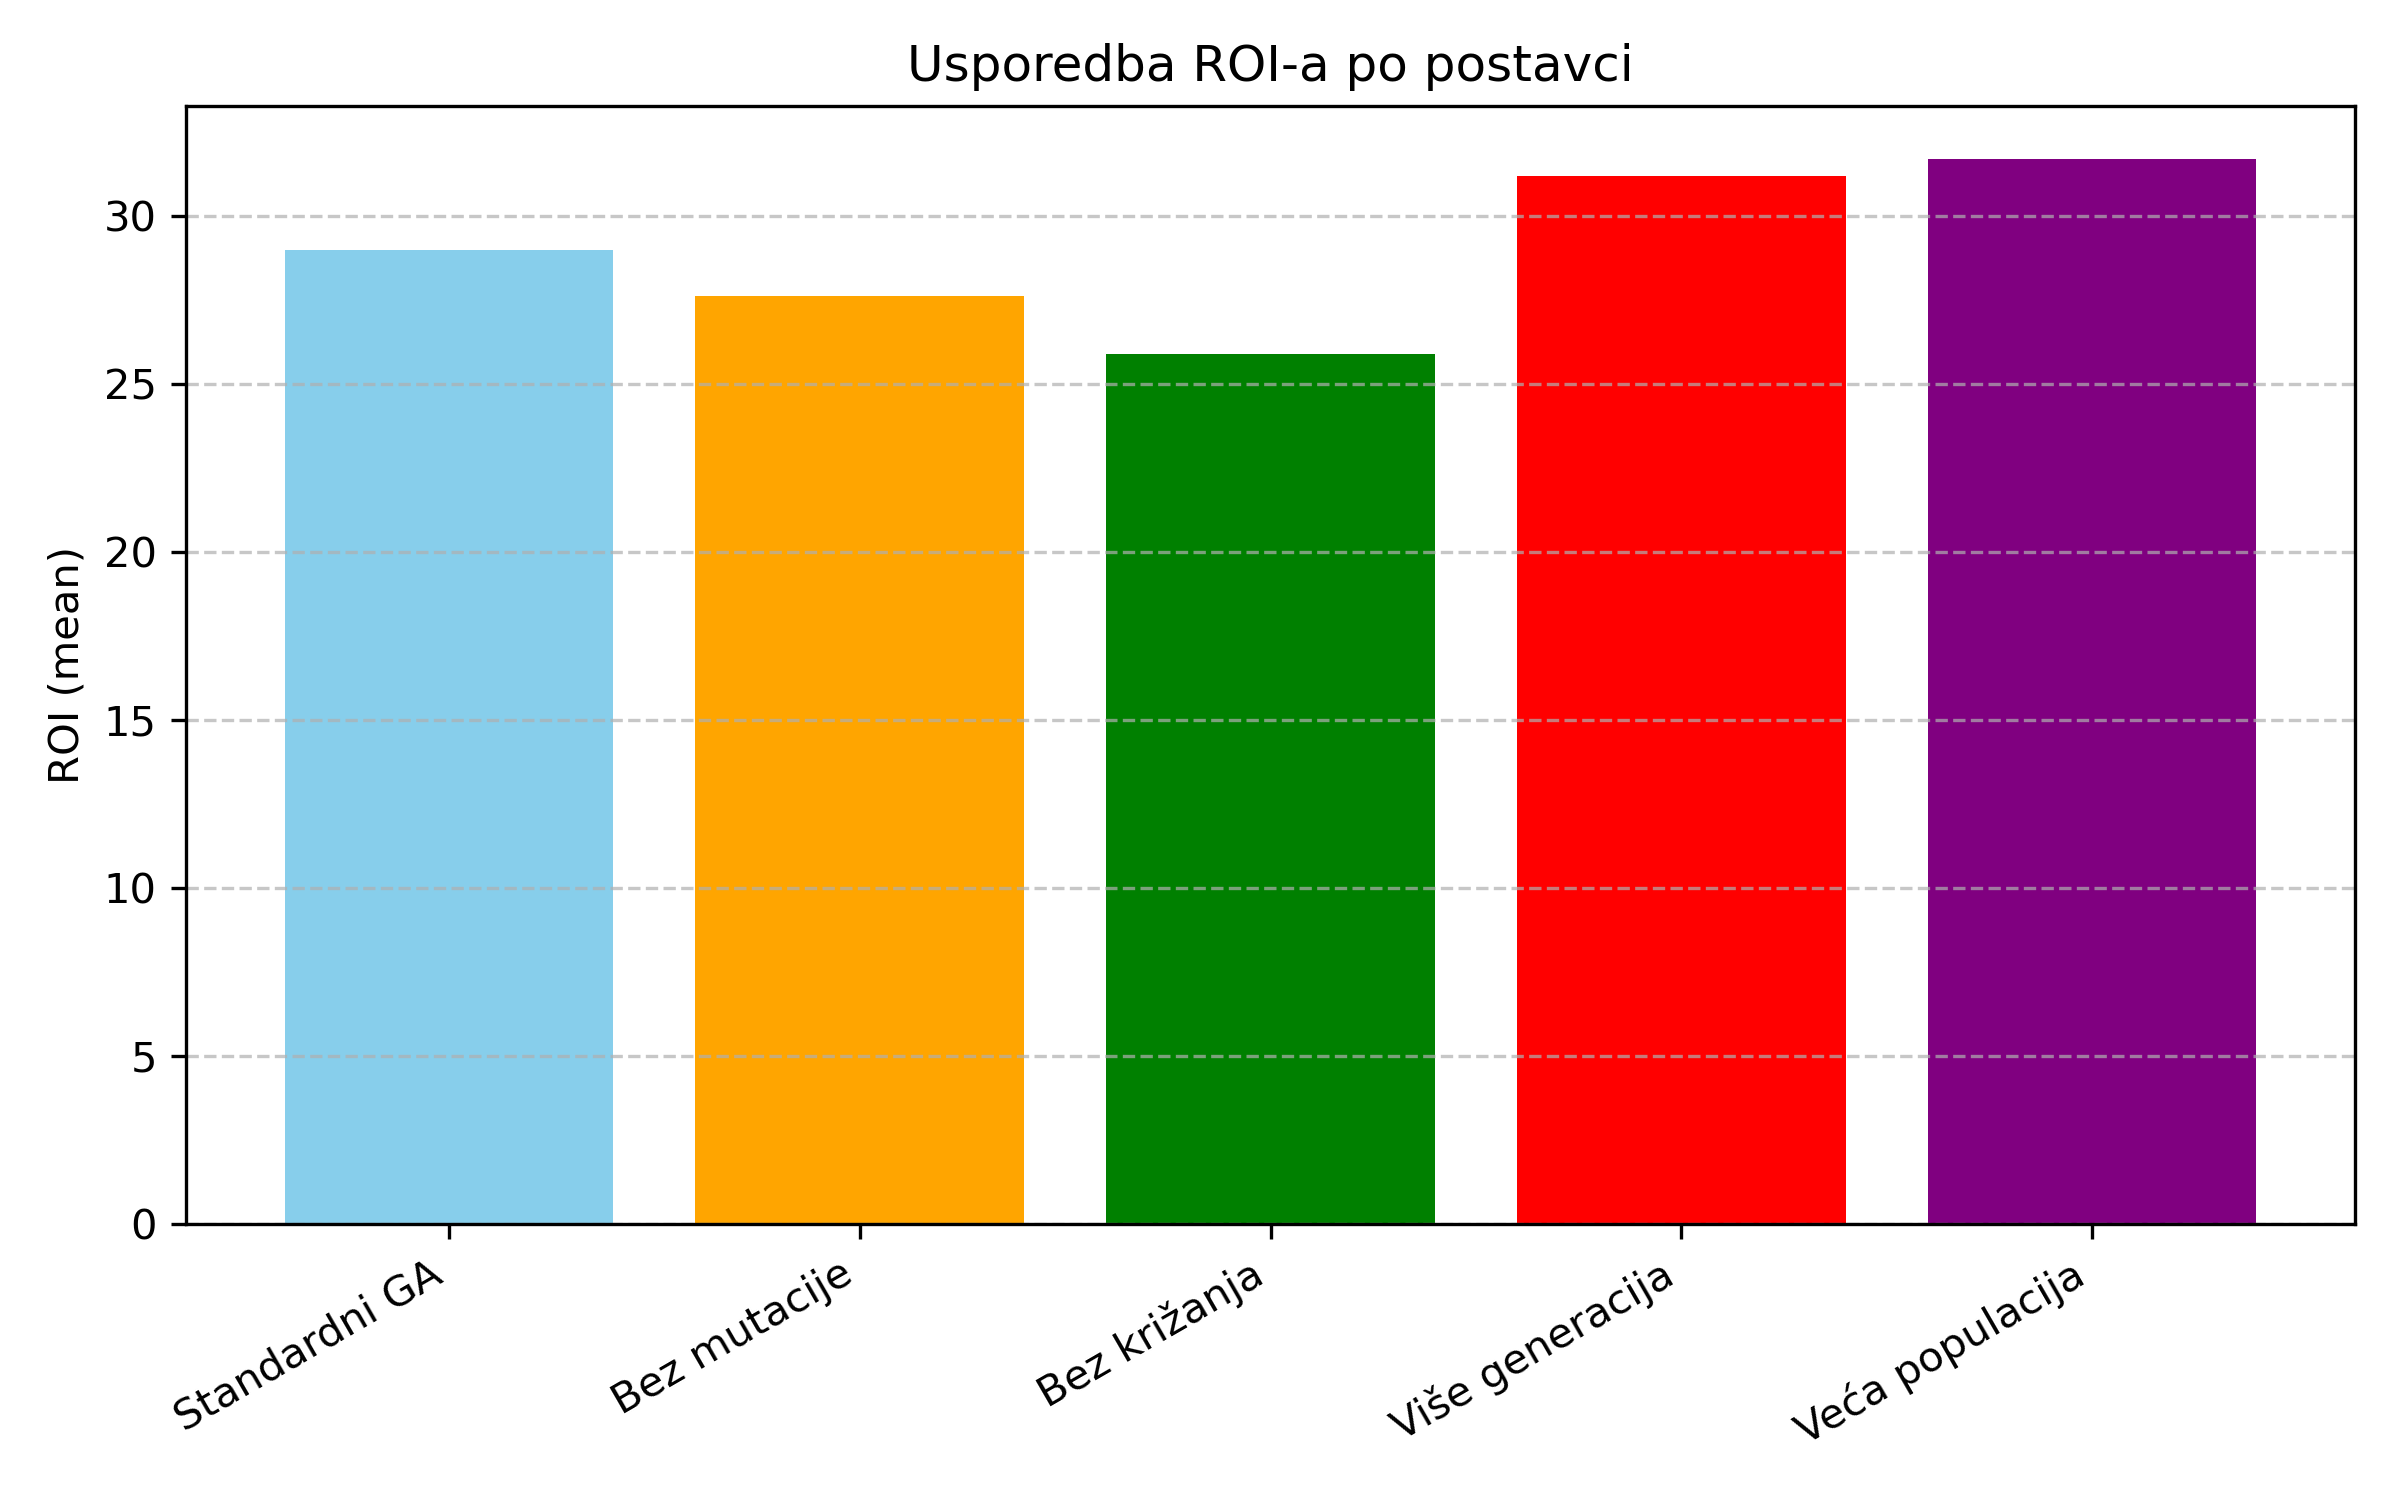
\includegraphics[width=\textwidth]{slike/ga_usporedba_roi.png}
        \caption{Usporedba prosječnog ROI-a za različite konfiguracije GA.}
        \label{fig:ga_roi}
    \end{subfigure}
    \hfill
    \begin{subfigure}[b]{0.48\textwidth}
        \centering
        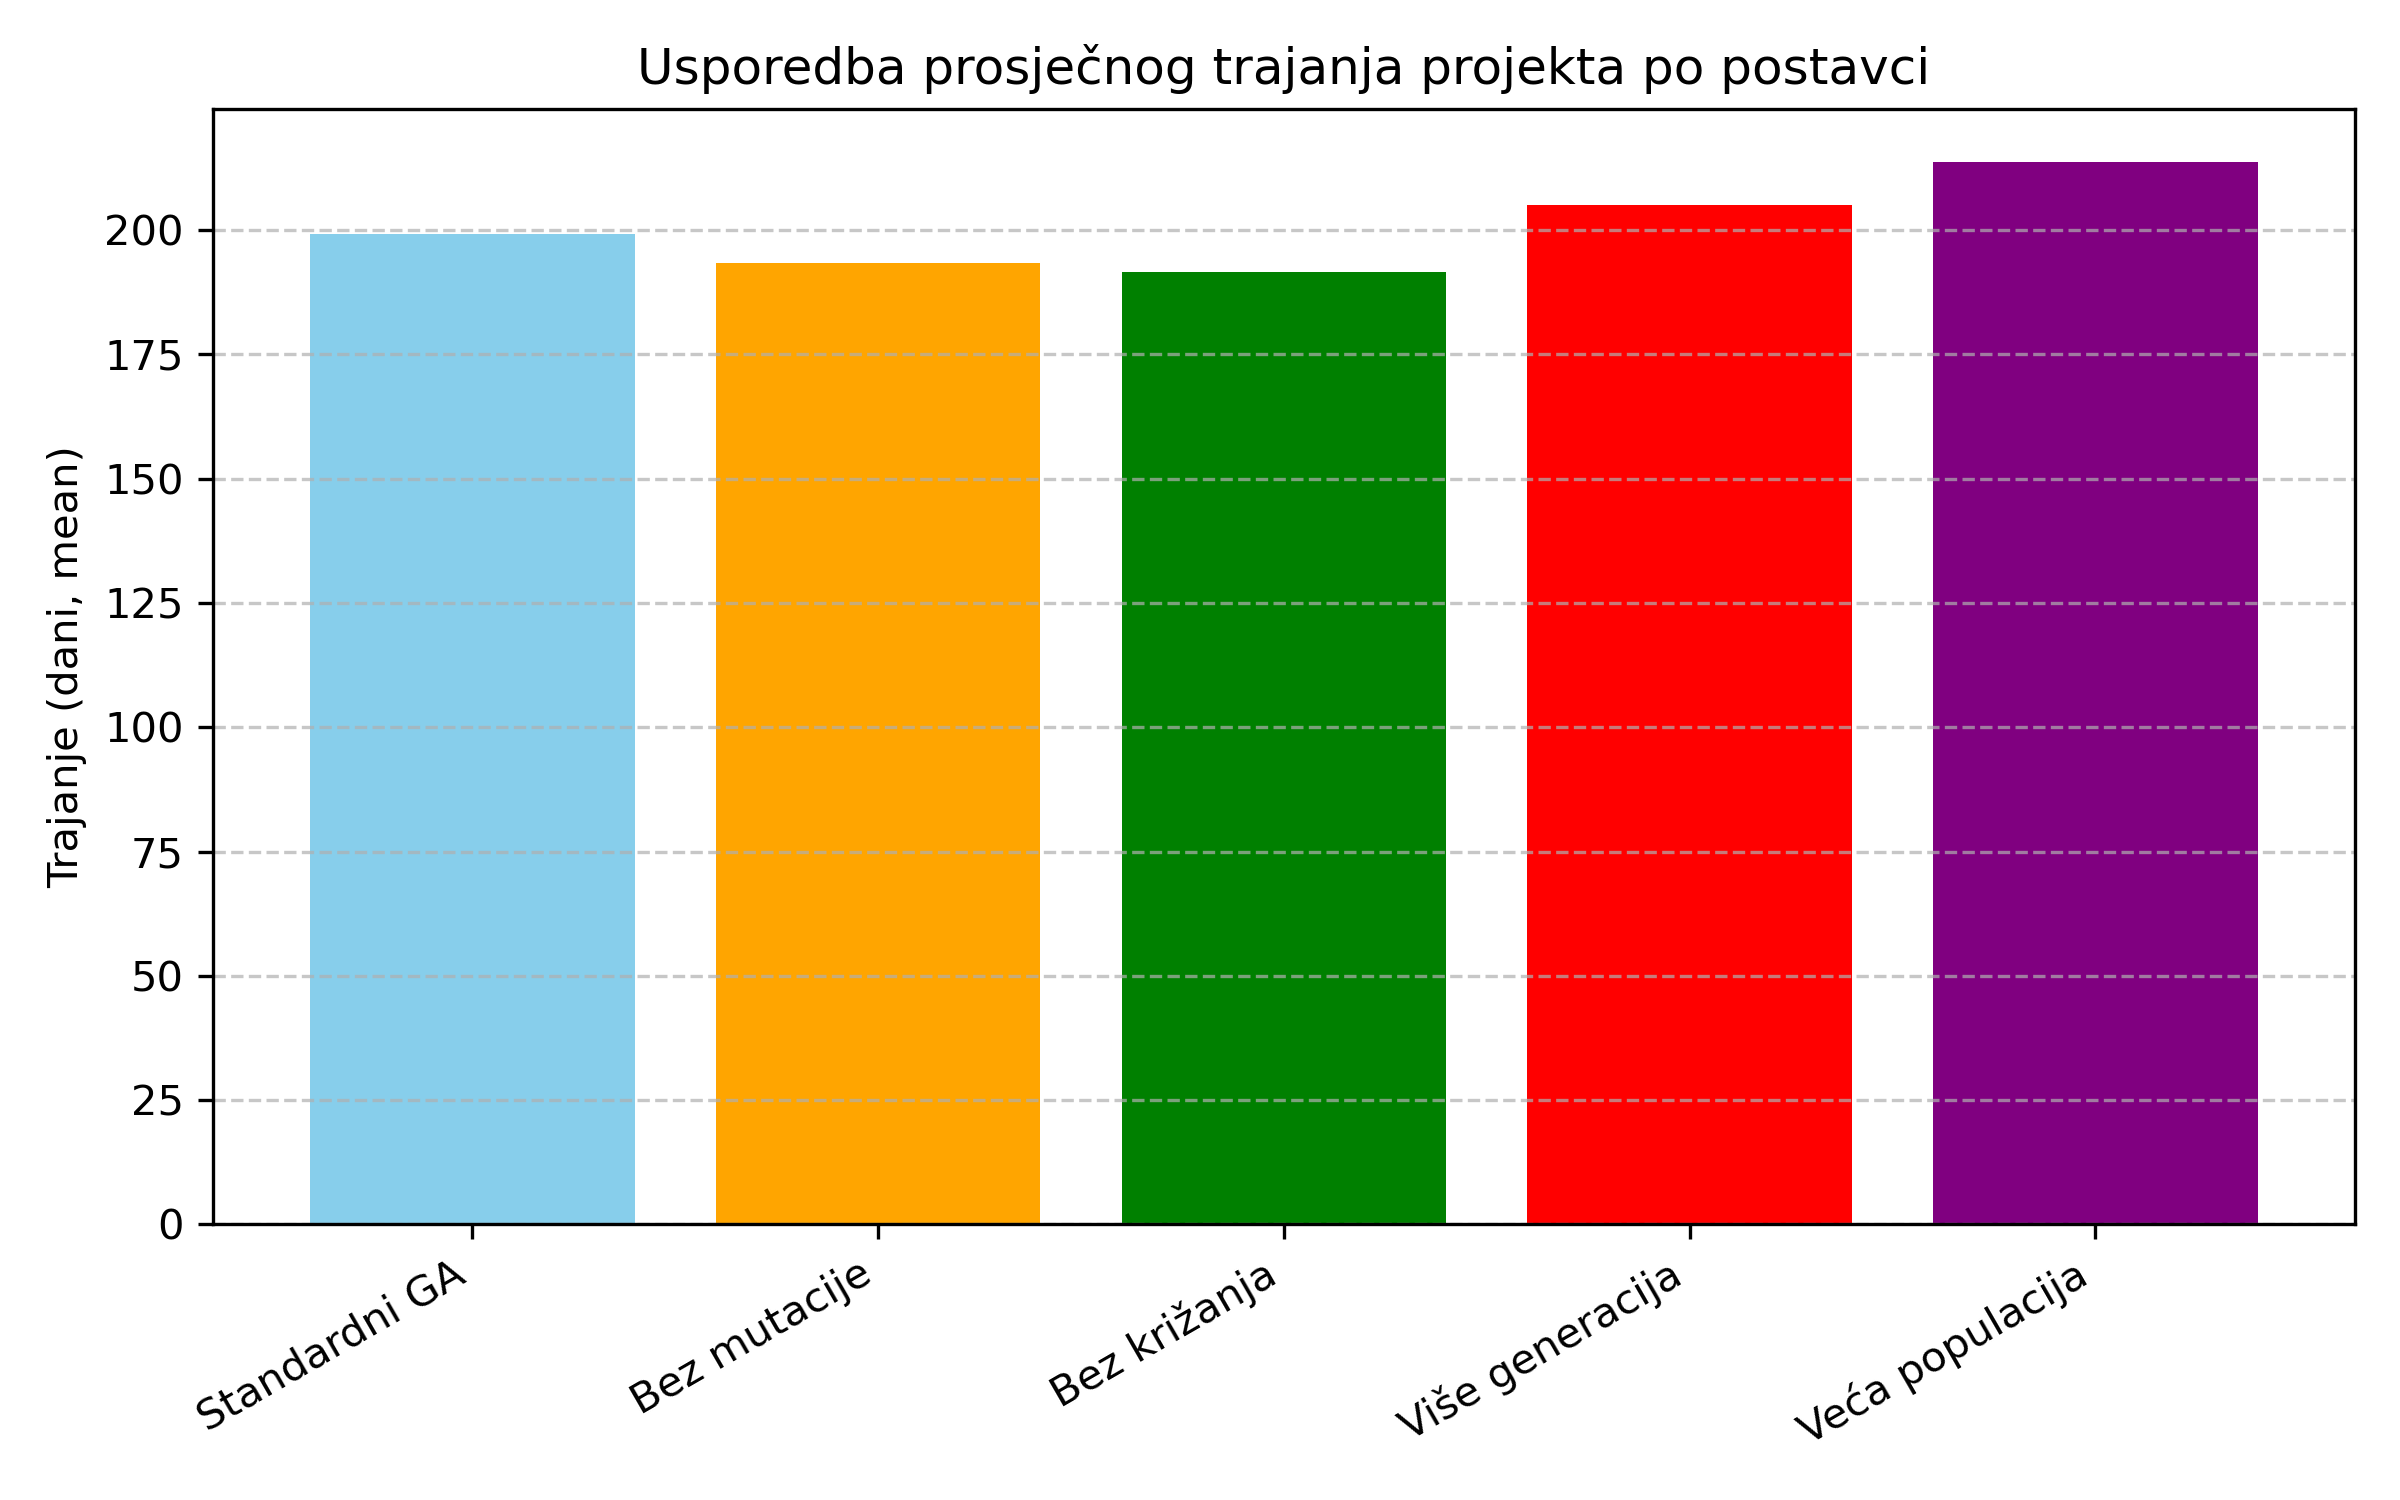
\includegraphics[width=\textwidth]{slike/ga_usporedba_trajanje.png}
        \caption{Usporedba prosječnog trajanja projekta za različite konfiguracije GA.}
        \label{fig:ga_trajanje}
    \end{subfigure}
    \caption{Grafički prikaz rezultata ablacijske studije za genetski algoritam.}
    \label{fig:ga_ablation}
\end{figure}

\textbf{Zaključak Eksperimenta 1:}  
Na temelju empirijskih rezultata, konfiguracija \emph{Veća populacija} odabrana je kao ``šampionska''. Njezini parametri (\texttt{POP\_SIZE = 200}, \texttt{NGEN = 40}, \texttt{CX\_PB = 0.7}, \texttt{MUT\_PB = 0.2}) koristit će se u svim daljnjim eksperimentima koji uključuju genetski algoritam, kako bi se osigurala njihova maksimalna učinkovitost i omogućila pravedna usporedba.

